\section{ETSI (European Telecommunications Standards Institute)}
ETSI\cite{ETSI} is a standardization organization in the telecommunications industry. Telecoms networks contain a large number of proprietary hardware and launch of new services often relied on on-site installation. In order to realize more flexibility for providing services ETSI proposed the NFV concept in 2012. Figure \ref{fig: ETSI_arc} shows the NFV architectural framework. The right box with dotted line represents the control plane and bigger box in the left with virtualized NFs atop describes NFV infrastructure installed in data plane. There is virtualization layer and virtual instances to support NFs because VM is used to realize NF. Detailed architecture is explained in the 2.2 section. 

\begin{figure*}
	\centering
	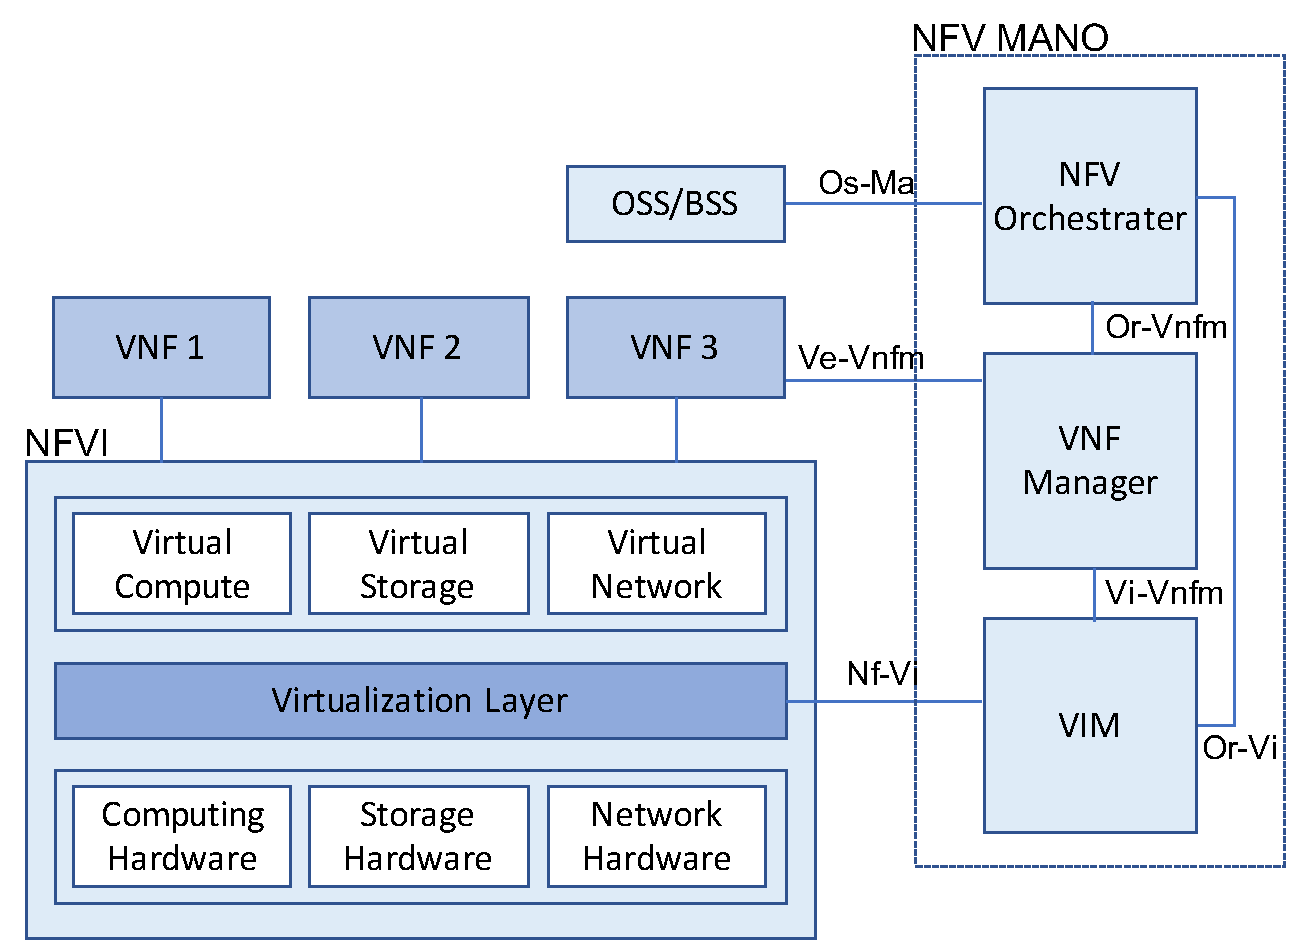
\includegraphics[width=100mm]{pics/ETSI_architecture.pdf}
	\caption{Architectural framework of NFV by ETSI.}
	\label{fig: ETSI_arc}
\end{figure*}

\section{OPNFV --- Open Platform for NFV}
\subsection{OPNFV: Architecture}
OPNFV\cite{OPNFV} is an open source project that realizes the architecture proposed by ETSI to provide carrier-grade, integrated platform for NFV. The OPNFV software platform is comprised of lot of projects and components related to NFV technologies. The architectural framework consists of the following 5 components. 
\begin{enumerate}
	\item Virtualised Network Function (VNF): One VNF may consists of multiple VMs, or in other cases, the whole VNF can be realized in a single VM.  
	\item Network Functions Virtualization Infrastructure (NFVI): NFVI has hardware and software part. Hardware NFVI corresponds to physical hardware such as servers, storage and network hardware. Software NFVI has 3 elements. First, virtual compute element which provides datapath for running VMs such as KVM. Secondly, virtual network element such as OVS, and thirdly virtual storage. 
	\item Virtual Infrastructure Management (VIM):  VIM controls and manages the interaction of a VNF with virtual compute, storage and network, as well as their virtualization. More specifically, it is in charge of allocating/releasing VMs on the hypervisors, increasing/decreasing resources to VMs. OpenStack, one of the largest open source projects in the world, is used as VIM in OPNFV. OpenStack itself is an umbrella project, containing numerous projects underneath. For example, Nova project for virtual compute service and Cinder project for virtual storage service are used in OpenStack.
	\item NFV Management and Orchestration (MANO) : Decoupling VNF from the underlying hardware resources requires an orchestrater that manages virtualization-specific tasks. It includes instantiating VNFs at appropriate locations, allocating hardware resources to the VNFs, keeping track of VNF instances location, etc. MANO is responsible of managing NFV infrastructure as described above to realizing network services. Following components manage virtual compute, networking, storage and VM resources. 
		\begin{itemize}
			\item NFV Orchestrater: Responsible for loading new network services and monitoring its lifecycle, and global resource management. As in Figure \ref{fig: ETSI_arc}, NFV orchestrater has interface between VNF Manager, VIM and OSS/BSS (Operation Support System / Business Support System). The first Or-Vnfm interface is used for VNF Manger to request virtual resources, and for NFV Orchestrater to send configuration information to VNF Manager so that VNF can be configured according to network service's demand. Or-Vi interface sends resource reservation/allocation requests by NFV Orchestrator. OSS/BSS is an interface that service provider operates through. 
			\item VNF Manager: Monitors lifecycle of VNF. Vi-Vnfm interface conveys resource allocation requests by VNF Manager to VIM. Ve-Vnfm interface is used for VNF lifecycle management and exchange of state information. 
		\end{itemize}
	\item Software Defined Networking (SDN) Controller: (SDN) Controller is control plane that is responsible for programming physical and virtual networking elements. SDN controller has northbound interface that connects with MANO and VIM, and southbound interface to physical and virtual networking switches. One of the southbound interface that is used is OpenFlow, which defines the communication protocol to enable SDN controller to directly interact with the forwarding plane. 
The aim of SDN controller in OPNFV is to set up overlay networks that connects VMs, so that NF chaining is accomplished. SDN controllers such as OpenDaylight\cite{OpenDaylight}, OpenStack Neutron and ONOS are integrated in OPNFV.
\end{enumerate}

A Network Service is described as a NF Forwarding Graph in OPNFV. NF Forwarding Graph has NF nodes connected with virtual link and underlying physical nodes connected with physical link. Figure 4 depicts an example of NF chaining. Forwarding Graph is composed of NF, VNF1, VNF2, ..,VNF4. Depending on the flow, traffic can go through NF chaining of NF1, NF3, NF4 or NF1, NF2, NF4. 
\begin{figure*}
	\centering
	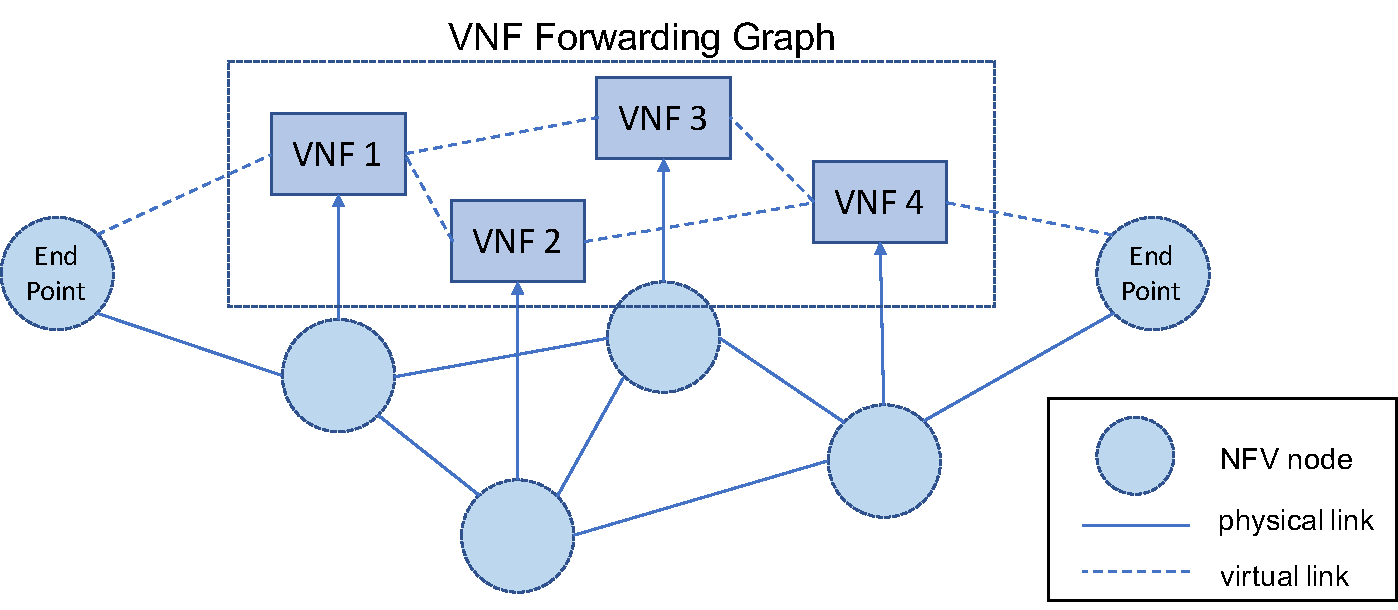
\includegraphics[width=120mm]{pics/NFV_FG.pdf}
	\caption{NFV Forwarding Graph}
	\label{fig: OPNFV_FG}
\end{figure*}

\subsection{Disadvantages of OPNFV}
Although OPNFV is a NFV platform that is widely deployed by enterprise and service provider, this thesis states the following two problems.
\begin{itemize}
	\item Complexity of OPNFV \\
		The architecture of OPNFV contains numerous middleware like OpenStack as a cloud controller, OpenDaylight as a SDN controller, KVM as virtual technologies, etc. Each of them are deriving from different project. This makes the architecture to be complicated and thus prone to compiling errors in different environments. 
	\item Resource consumption \\
		By allocating virtual instances to each of the VM, it leads to a lot of resource consumption when deploying a large number of VMs. 
	\item Memory copy \\
		Delivering packets to NFs causes memory copy because NFs are virtualized instances running in the user space. With heavy traffic this packet forwarding can be the bottleneck to maintain throughput. 
	\item Scaling problem of OPNFV \\
		OPNFV uses NFV Forwarding Graph to achieve NF chaining. SDN controller like OpenDaylight installs flow classifier in each NFV node. And OVS in NFV node forwards traffic according to the installed classifier, such as passing packets through NF on its node or transmitting packets to another node. Since a SDN controller is responsible for setting up service chain, it is not realistic to be deployed in wide area network. 
\end{itemize}

\section{Flurries: Countless Fine-Grained NFs for Flexible Per-Flow Customization} 
Flurries\cite{flurries} is a container-based NFV platform designed to support large number of lightweight NFs. This thesis argues that even though SDN enables fine grained routing, this flexibility of flow cannot be extended to network function layer because packets of all flows are aggregated in a queue before processing. Each NF receives packets of many different flows and it is NF's responsibility to divide those packets into flows. This thesis proposes that for each flow a NF should run to provide QoS and service chain functionality per flows at a very fine granularity. To add flexibility, a NF is broken down into pieces of single service, "microservice". In order to run a large number of NFs on a single host, a microservice is realized by a lightweight container. 

\begin{figure*}
	\centering
	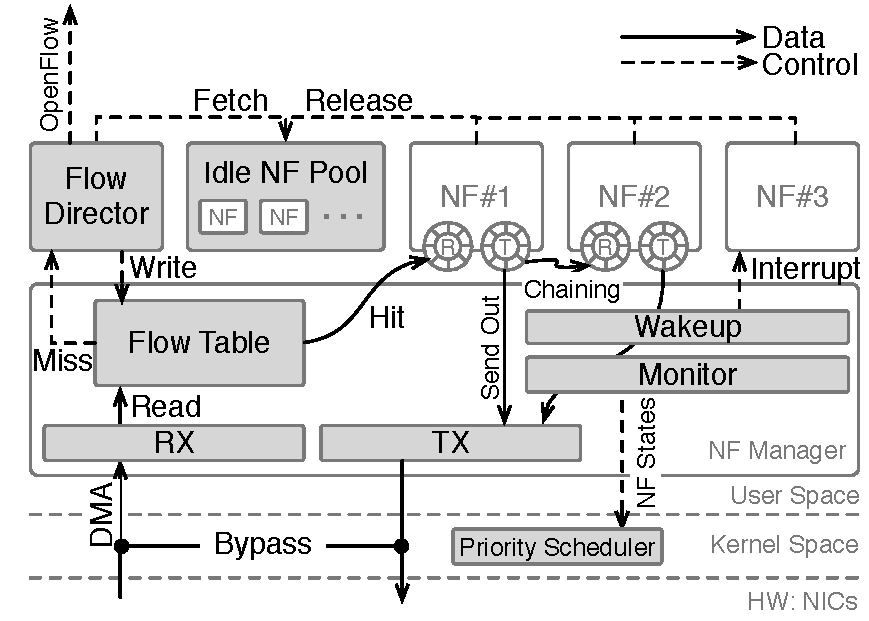
\includegraphics[width=95mm]{pics/flurries_arc.pdf}
	\caption{Architecture of Flurries}
	\label{fig: flurries_arc}
\end{figure*} 

Flurries's architecture is shown in Figure \ref{fig: flurries_arc}. Flurries uses DPDK to bypass kernel and directly access DMA\cite{DMA} (Direct Memory Access) of the NIC. Flurries Manager is the big box in the middle that is responsible for fetching packets from the NIC and forward them to the right containers as marked NF\#1, NF\#2 and NF\#3. When packets arrive at the NIC, the RX threads in the Flurries Manager use DPDK's poll mode driver to read packets into a memory region shared with all NFs. Then the RX thread performs lookup in the Flow Table and if there is a match the packet descriptor is copied into the the NF's receive buffer.  

There are following common elements in Flurries and in my Kernel-based NFCI.
\begin{itemize}
	\item Zero copy: In Flurries, packets are collected in a shared memory where all the NFs can access so that packets do not need to be copied to NFs for the process. Kernel-based NFCI realizes zero copy as well by chaining NFs inside the kernel where only single memory region exist. 
	\item Microservice: In Flurries, a NF is fragmented to pieces of a single service that work in containers. In Kernel-based NFCI, NFs are implemented with kernel modules and a NF can consist of several modules. This also makes it possible to break down a NF into several services (kernel modules) and share the common service among NFs to reduce redundancy in NFs. 
\end{itemize}

Big difference between Flurries and Kernel-based NFCI is how zero copy is realized. Flurries bypasses the network stack by using DPDK to directly access DMA, whereas Kernel-based NFCI realize zero copy by operating in the network stack. 

Although problem of memory violation arises when using DPDK to bypass the OS. The NF Manager uses DPDK Packet Distributor library to fetch packets and store them in a shared memory. And all the containers can access to this data packet even though there are certain containers that should not be allowed to see them. Originally applications in the user space cannot see data that are destined to other applications, which is realized by socket API. However if the kernel stack is bypass it is impossible to obtain security provided by the kernel. This is a harmful effect caused by raising the function of memory management to user space which kernel should originally control. This is not limited to Flurries but to all the NFV platform that using bypassing technology for better throughput. 

For such reason I propose a secure NF chaining infrastructure in kernel without using bypass technology like DPDK. 






